%%%%%%%%%%%%%%%%%%%%%%%%%%%%%%%%%%%%%%%%%%%%%%%%%%%%%%%%%%%%%%%%%%%%%%%%
%  Sección 2.2 - Ejemplo con trazas
%%%%%%%%%%%%%%%%%%%%%%%%%%%%%%%%%%%%%%%%%%%%%%%%%%%%%%%%%%%%%%%%%%%%%%%%

\section{Ejemplo con trazas}
En este caso, vamos a explicar el uso de una herramienta que puede ser útil a la hora de depurar un circuito, ya que nos permite visualizar el diagrama de ondas de las señales. Tal vez para este ejemplo tan pequeño, la depuración por este medio puede no ser la más rápida, pero nos permitira ilustrar fácilmente su funcionamiento. En este caso, vamos a diseñar un multiplexor que envíe a la salida una de entre cuatro entradas, es decir, un mux 4:1. El código se muestra en el listing \ref{lst:ejemplo-con-traza}.

\lstinputlisting[style=verilogstyle, label=lst:ejemplo-con-traza, caption={Multiplexor 4 a 1.}]{codigo/ejemplo-con-traza/top.sv}

% Subsección 2.2.1 - verilar 
\subsection{Verilar}
La verilación del circuito es igual que en el ejemplo básico exceptuando la adición de la opción \verb|--trace| que creará el código en C++ necesario para la generación de diagramas de ondas. El comando a ejecutar se muestra en el Listing \ref{lst:verilar-traza}.

\begin{mycode}[style=bashstyle, label=lst:verilar-traza, caption={Instrucción para verilar el diseño habilitando las trazas.}]
verilator -Wall --trace -cc inversor.sv
\end{mycode}

% Subsección 2.2.2 - envolver 
\subsection{Envolver}
La idea a seguir a la hora de programar el banco de pruebas es la misma que en el caso anterior (y en todos los casos): crear una función \verb|main| dentro de la cual programaremos un bucle que estimule el modelo verilado y lo evalue en cada flanco de subida del reloj. No obstante, para crear el fichero con la información necesaria para visualizar el diagrama de ondas hay que instanciar un objeto concreto que nos permitirá volcar la información en dicho fichero. 

En el Listing \ref{lst:tb-ejemplo-con-traza}, se puede ver como, tras la instanciación del modelo verilado, instanciamos el objeto \verb|VerilatedVcdC| llamándolo \verb|tfp| (nótese que hay que incluir el fichero de cabecera correspondiente al principio), y que contiene las funciones necesarias para la creación del fichero que abriremos con un programa de visualización de diagramas de ondas (GTKWave) y para el volcado del estado de las señales en dicho fichero. En la línea 34, pasamos dicho objeto a la función \verb|trace| del modelo verilado, de manera que este quede asociado a dicho modelo y trace sus señales. El 99 indica los niveles de jerarquía que queremos trazar. Cada nivel se corresponde con la instanciación de un módulo dentro del módulo que se quiere trazar, de tal modo que si el módulo \verb|top.sv| instancia un módulo \verb|m1.sv| y este a su vez un módulo \verb|m2.sv|, la jerarquía tendrá 2 niveles. Con un valor de 99 nos aseguramos de que todas las señales del circuito se tracen, ya que es muy difícil que un diseño tenga tantos niveles de jerarquía. En la línea 35, utilizamos el objeto \verb|tfp| para abrir el fichero en el que volcaremos los datos de las señales durante la simulación. La ruta que se le pasa entre paréntesis es relativa, de tal manera que dicho fichero se guardará en el directorio donde se encuentre el banco de pruebas. Para volcar los datos de las señales en un momento dado, se usa la función \verb|dump| del objeto \verb|tfp|. Para indicar el tiempo de simulación que queremos volcar, pasamos el valor devuelto por la función \verb|time| del contexto de la simulación. Finalmente, antes de liberar el modelo verilado, cerramos el fichero con los datos de los diagramas de ondas (línea 74).

\begin{center}
	\lstinputlisting[style=verilogstyle, label=lst:tb-ejemplo-con-traza, caption={Banco de pruebas para el ejemplo con traza.}]{codigo/ejemplo-con-traza/tb_top.cpp}
\end{center}


% Subsección 2.2.3 - compilar 
\subsection{Compilar}
La compilación del banco de pruebas es muy similar también al ejemplo básico, pero incluyendo un fichero nuevo que hay que compilar. El fichero extra que hay que compilar es el que implementa las funciones indicadas en el fichero de cabecera que incluimos en el banco de pruebas: \verb|verilated_vcd_c.h|. Si se ha instalado Verilator de la manera estándar, dicho fichero se debería encontrar en \linebreak\verb|/usr/share/verilator/include/verilated_vcd_c.cpp|. De este modo, el comando para compilar quedaría de la manera que se muestra en el Listing \ref{lst:compilar-tb-traza}.

\begin{mycode}[style=bashstyle, label=lst:compilar-tb-traza, caption={Compilación del banco de pruebas incluyendo el fichero necesario para crear trazas.}]
g++ -I /usr/share/verilator/include/ -I obj_dir/ /usr/share/verilator/include/verilated_threads.cpp /usr/share/verilator/include/verilated.cpp /usr/share/verilator/include/verilated_vcd_c.cpp tb_top.cpp obj_dir/Vtop__ALL.a -o Vtop
\end{mycode}

% Subsección 2.2.4 - simular 
\subsection{Simular}
Si la compilación es exitosa, se debería crear el ejecutable \verb|Vtop| que, tras su ejecución, debería mostrar en la salida estandar los resultados de la simulación y generar un fichero llamado \verb|simx.vcd| y que es el que utilizaremos abriremos con el programa GTKWave para visualizar el diagrama de ondas.

% Subsección 2.2.5 - depurar 
\subsection{Depurar}
Para depurar de una manera más visual, o seleccionar sólo un subconjunto del total de señales del circuito, vamos a utilizar el visualizador de diagramas de ondas GTKWave. Dicho programa se lanza desde la terminal, pasándole como argumento el fichero \verb|.vcd| que hemos generado durante la simulación (véase el Listing \ref{lst:depurar}).

\begin{mycode}[style=bashstyle, label=lst:depurar, caption={Instrucción para lanzar el programa de visualización de diagramas de ondas.}]
gtkwave simx.vcd
\end{mycode}

En la Figura \ref{fig:gtkwave-ejemplo-con-traza} se muestra el programa en ejecución. En él se han seleccionado todas las señales del circuito y se han insertado en el panel principal para su visualización.

\begin{figure}[htb]
	\centering
	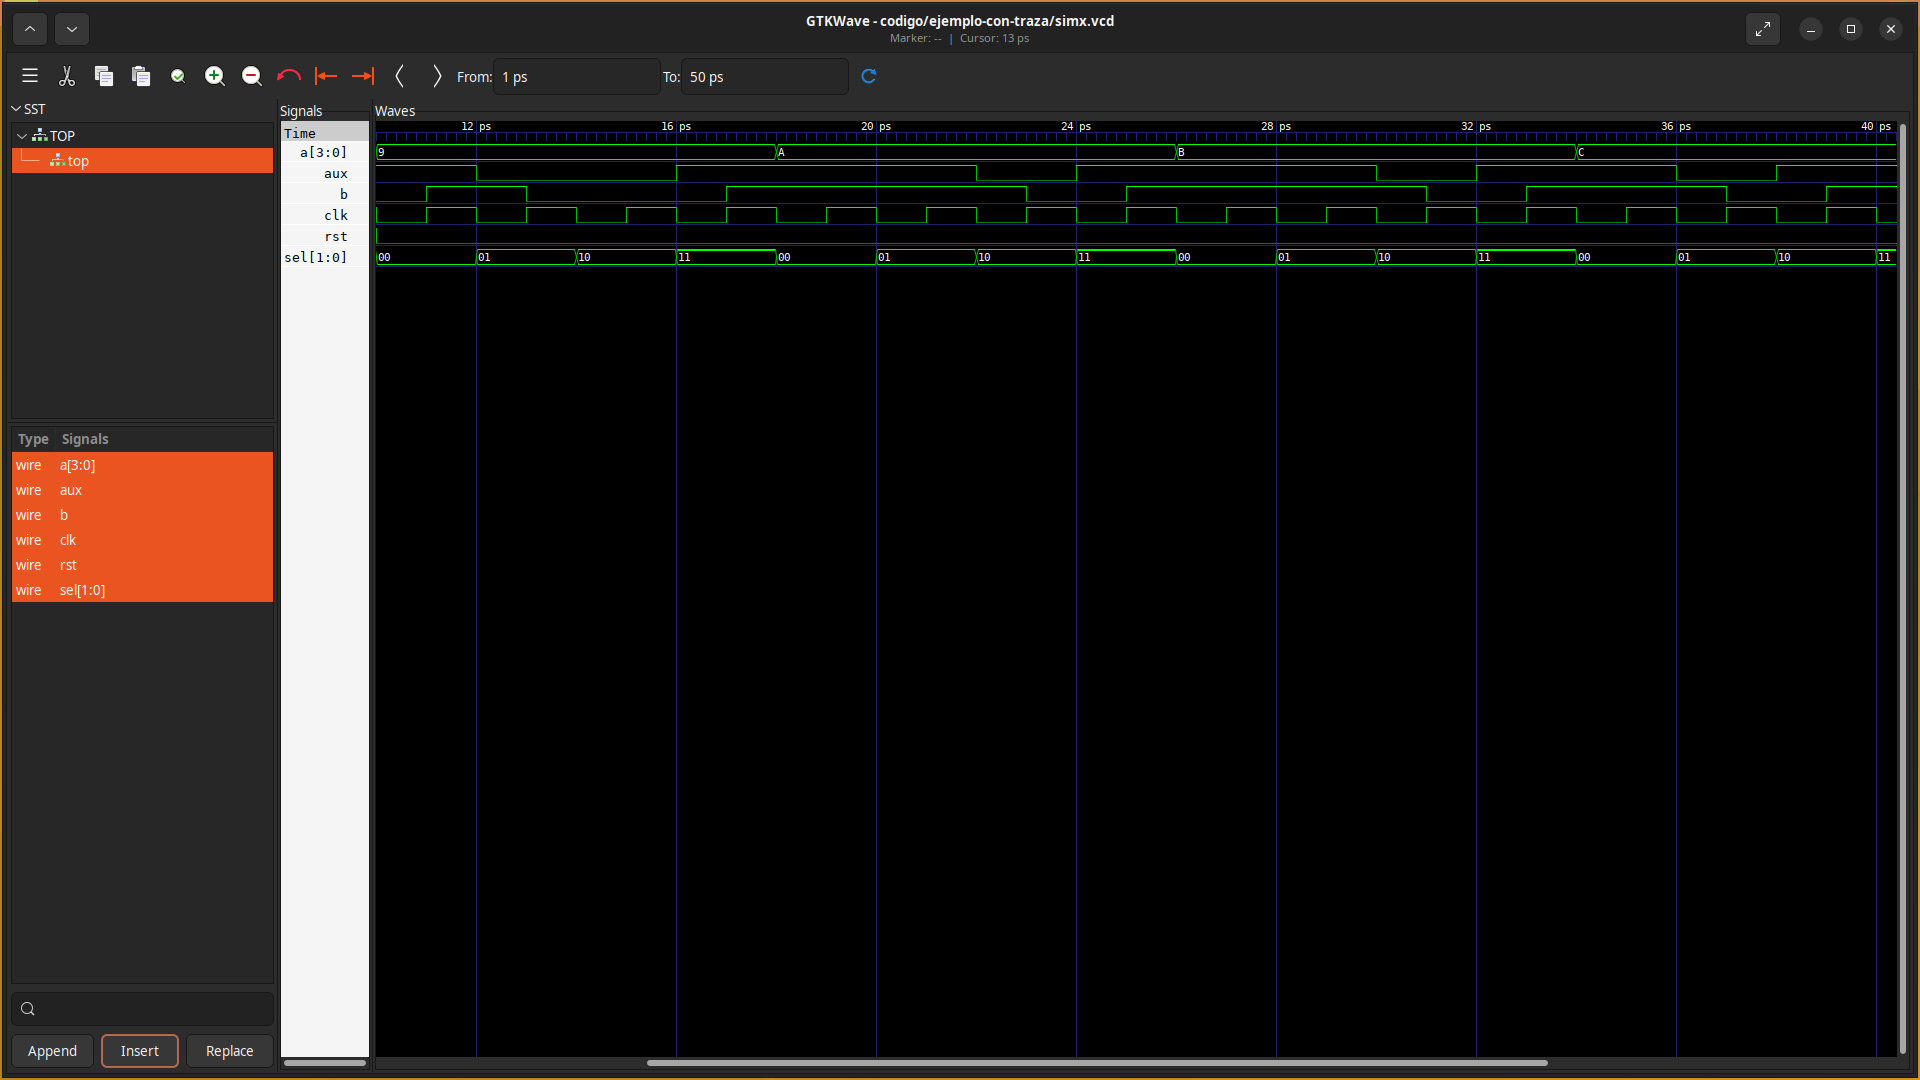
\includegraphics[width=\textwidth]{figs/gtkwave-ejemplo-con-traza.png}
	\caption{GTKWave.}
	\label{fig:gtkwave-ejemplo-con-traza}
\end{figure}
